\documentclass[12pt]{article}

\usepackage{amssymb,amsmath,amsfonts,bbm,eurosym,geometry,ulem,graphicx,caption,color,setspace,sectsty,comment,footmisc,caption,natbib,pdflscape,subfigure,array,hyperref, booktabs, tabularx}

\usepackage[T1]{fontenc}
\usepackage[utf8]{inputenc}
\usepackage{babel}
\usepackage[font=small,labelfont={bf,sf},tableposition=top]{caption}

\normalem

\onehalfspacing
\newtheorem{theorem}{Theorem}
\newtheorem{corollary}[theorem]{Corollary}
\newtheorem{proposition}{Proposition}
\newenvironment{proof}[1][Proof]{\noindent\textbf{#1.} }{\ \rule{0.5em}{0.5em}}

\newtheorem{hyp}{Hypothesis}
\newtheorem{subhyp}{Hypothesis}[hyp]
\renewcommand{\thesubhyp}{\thehyp\alph{subhyp}}

\DeclareMathOperator\erfc{erfc}

\newcommand{\red}[1]{{\color{red} #1}}
\newcommand{\blue}[1]{{\color{blue} #1}}

\newcolumntype{L}[1]{>{\raggedright\let\newline\\arraybackslash\hspace{0pt}}m{#1}}
\newcolumntype{C}[1]{>{\centering\let\newline\\arraybackslash\hspace{0pt}}m{#1}}
\newcolumntype{R}[1]{>{\raggedleft\let\newline\\arraybackslash\hspace{0pt}}m{#1}}

\geometry{left=1.0in,right=1.0in,top=1.0in,bottom=1.0in}

\begin{document}

\begin{titlepage}
\title{The replicating portfolio of a constant product market}
\author{Joseph Clark\thanks{RMIT Blockchain Innovation Hub. joecmail@gmail.com} }
\date{\today}
\maketitle
\begin{abstract}
\noindent We derive the replicating portfolio of a constant product market. This is structurally short volatility (selling options) which explains why positive transaction costs are needed to induce liquidity providers to participate. Where futures and options markets do not exist, this payoff can be used to create them.

%\vspace{0in}\\
%\noindent\textbf{Keywords:} key1, key2, key3\\
%\vspace{0in}\\
%\noindent\textbf{JEL Codes:} key1, key2, key3\\

\bigskip
\end{abstract}
\setcounter{page}{0}
\thispagestyle{empty}
\end{titlepage}
\pagebreak \newpage




\doublespacing


\section{Introduction} \label{sec:introduction}

A constant product market (CPM) is a mechanism to trade between pairs of assets. A typical CPM is a pool containing a quantity of both assets with a rule specifying the amount of one asset that will be exchanged for another. Arbitrage with external spot markets ensures that the ratio of the quantities of assets in the pool should be close to the prevailing exchange rate. 

Liquidity providers put up the pool of assets and are able to redeem at any time, receiving a proportion according to the new ratio of assets as well as a share of transaction fees. It can be shown that the payoff to liquidity providers is proportional to the square root of the exchange rate between the two assets (see  \cite{ang20}). This payoff can be replicated precisely with a static combination of futures and options. If these futures and options exist and are tradable, the transaction fee charged by the CPM will be determined by the option prices and the expected quantity of transactions. If the options do not exist the payoff of the CPM can be used to create them.

% Might be nice to do a model of the tcost using expected transaction quantities

This second replication of European options with the CPM payoff is a novel use of these contracts, and one that has potential application to support new option markets without requiring traditional option market makers. 

\section{Preliminaries}

For the most part we follow the notation of \cite{ang20} who examine constant product markets such as Uniswap.


\textbf{Definition 1: Constant product market}

A constant product market (CPM) is a tuple $(t, R_\beta, R_\alpha)$. A transaction depositing $\Delta_\beta$ at time $t$ will receive $\Delta_\alpha$ satisfying

\begin{equation} \label{CPM}
(R_\alpha - \Delta_\alpha)(R_\beta + \Delta_\beta) = k
\end{equation}

Where $R_\beta,R_\alpha >0$,  $k=R_\alpha R_\beta$. Reserves are updated according to $R_\beta \mapsto R_\beta + \Delta_\beta$, $R_\alpha \mapsto R_\alpha - \Delta_\alpha$.

For simplicity the initial reserves are exogenous.


\textbf{Definition 2: Spot market}

A spot market is a mechanism which exchanges $\Delta_\alpha$ units of $\alpha$ for $m_p^t\Delta_\beta$ units of $\beta$ at time $t$. An infinitely elastic spot market is one where $m_p^t$ does is not depend on $\Delta_\beta$

\section{The value of a constant product market}

Summarising the development in Aegeris (2019) let $m_p^t$ be the price in the spot market. No arbitrage  gives $m_p^t = R_\beta^t/R_\alpha^t$. Combining with \ref{CPM} gives 

\begin{equation}
R_\beta^t= \sqrt{km_p^t}
\end{equation}

The return between two periods is

\begin{equation*}
\delta^t= \frac{m_p^t R_\alpha^t + R_\beta^t }{m_p^{t-1} R_\alpha^{t-1} + R_\beta^{t-1}} 
\end{equation*}

Substitute for $m_p^t$ and then for $R_\beta^t$

\begin{equation*}
\delta^t= \frac{R_\beta^t }{R_\beta^{t-1}} = \sqrt{\frac{m_p^t}{m_p^{t-1}}}
\end{equation*}


The total gain in the portfolio value is

\begin{equation*}
\delta = \prod_{t=2}^T \delta^t  = \sqrt{\frac{m_p^T}{m_p^1}}
\end{equation*}


The final portfolio value is the initial portfolio inflated by the gain

\begin{equation*}
P_V^T = (m_p^1 R_\alpha^1 + R_\beta^1) \delta = 2 \sqrt{km_p^T}
\end{equation*}


\section{The replicating portfolio for the CPM}

To replicate $P_V^T$ we use the spanning result of Green and Jarrow (1987) which provides that any function $W$ of a final price $m^T$ can be replicated as

\begin{equation} \label{SpanningResult}
W(S^T) = W(A)e^{-rT} + W'(A)(m^T -Ae^{-rT}) + \int_0^A W''(K) P(K) dK +   \int_A^\infty W''(K) C(K) dK
\end{equation}

Where $r$ is the interest rate (from here we'll assume $r$=0). We choose $A = m^0$ (suppressing the subscript) and replicate with a bond, futures, and strips of options on the underlying all expiring at $T$:

\begin{eqnarray*}
\hbox{Face value of bond:   }&  W(m^0) =& 2 \sqrt{km^0}\\
\hbox{Notional value of futures:   }& W'(m^0) =& \sqrt{\frac{k}{m^0}}\\
\hbox{Notional value of options at strike $K$:   }& W''(K) =& -  \frac{1}{2} \sqrt{\frac{ k}{K^3}} dK
\end{eqnarray*}

The appendix has an example of replication with limited strikes.


\section{Replicating European options from with the CPM}

We now replicate in the other direction -- creating a European call option from a CPM. Unlike the previous replication this is neither perfect or static, though it can be made quite precise even with limited re-hedging (see Appendix B).

Say we have a European call option expiring at $T$ and the payoff of the CPM. We have use of the following greeks:

\begin{eqnarray*}
\hbox{CPM delta:   }& \text{Delta}_{CPM}^t =& \frac{\partial CPM^t }{\partial m^t} =  \sqrt{\frac{k}{m^t}}\\
\hbox{CPM gamma   }& \Gamma_{CPM}^t =& \frac{\partial^2 CPM^t }{(\partial m^t)^2} = -  \frac{1}{2} \sqrt{\frac{ k}{(m^t)^3}}\\ 
\hbox{Call delta:   }& \text{Delta}_{C}^t =&  \frac{\partial C^t }{\partial m^t}  & \\
\hbox{Call gamma   }& \Gamma_{C}^t  =& \frac{\partial^2 C^t }{(\partial m^t)^2} & \\
\hbox{Call theta   }& \Theta_{C}^t =& \frac{\partial C^t }{\partial t}  & 

\end{eqnarray*}

 We can replicate by matching exposures to the underlying. The hedge ratio to match the gamma of the CPM and the call option is 

\[HR^t = \frac{\Gamma_C^t}{\Gamma_{CPM}^t} \]

The payoff of the call can be approximated with  

\begin{equation}
\label{VC}
\Delta V_C^t \approx \text{Delta}_C \Delta m^t + 0.5 \Gamma_C^t (\Delta m^t)^2   + \Theta_C^t \Delta t    
\end{equation}


The delta and gamma components can be approximated by holding combination of the CPM and a futures contract on $m^t$. The replicating portfolio is:


\begin{eqnarray*}
\hbox{Notional value of futures:   }& \text{Delta}_C^t - HR^t \text{Delta}_{CPM}^t \\
\hbox{Notional value of CPM:   }& HR^t
\end{eqnarray*}

The payoff is

\begin{equation}
\label{VCPrime}
 \Delta V_{C'} - \Theta_C^t \Delta t  = HR^t \Delta CMP^t + \left(\text{Delta}_C^t - HR^t \text{Delta}_{CPM}^t \right) \Delta m^t    
\end{equation}

Appendix B demonstrates the accuracy of the replicating portfolio for an at-the money call with simulated prices. 


\section{Discussion}

The existence of a static replicating portfolio for the CPM means that the payoff can be perfectly hedged. In this case the transaction fee will be determined by these option prices combined with an expectation of transaction quantity. On the other hand if there are no option and futures markets, or if they are not tradeable, the payoff of the CPM itself can be used to replicate the options. 

%If there are no underlying option markets, the price will be determined by market preferences for variance. The replicating portfolio sells a strip of options on the exchange rate $m_p^T$. The delta hedged replicating portfolio payoff is decreasing in the variance of  $m_p^t$. Risk averse investors have decreasing utility in variance and would require a premium to sell these options (see \cite{CarrWu09}). Equally, equity holders in the CPM will equally require compensation via a positive transaction fee for the options embedded in their payoff.   

%It's notable that the replicating portfolio bears a passing resemblance to the $1/K^2$ strikes used to replicate the log contract needed for a variance swaps (see \cite{Derman99}}.





\singlespacing
\setlength\bibsep{0pt}
\bibliographystyle{my-style}
\bibliography{Placeholder}



\clearpage

\onehalfspacing

%\section*{Tables} \label{sec:tab}
%\addcontentsline{toc}{section}{Tables}



%\clearpage

%\section*{Figures} \label{sec:fig}
%\addcontentsline{toc}{section}{Figures}

%\begin{figure}[hp]
%  \centering
%  \includegraphics[width=.6\textwidth]{../fig/placeholder.pdf}
%  \caption{Placeholder}
%  \label{fig:placeholder}
%\end{figure}




\clearpage

\section*{Appendix A. Example: Replicating a CPM with options} \label{sec:appendixa}


Consider a constant product market with state 

\[(t, R_\beta, R_\alpha) = (1, 10, 200)\] 

The price of $\beta$ in units of $\alpha$ is $m_p^1 = \frac{R_\beta}{R_\alpha} = 0.05$.

The initial value of the pool (in units of $\beta$) is

\[P_V^1 = (m_p^1 R_\alpha^1 + R_\beta^1) = 0.05*200+10 = 20\]

The replicating portfolio is: 

\begin{eqnarray*}
\hbox{Face value of bond:   }&  W(m_p^0) &= 2 \sqrt{km_p^0} = 2\sqrt{2000*0.05} = 20\\
\hbox{Notional value of futures :   }& W'(m_p^0) &= \sqrt{\frac{k}{m_p^0}} = \sqrt{\frac{2000}{0.05}} = 200 \\
\hbox{Notional value of options at strike $K$} & W''(K) &= -  \frac{1}{2} \sqrt{\frac{ k}{K^3}} dK = \frac{0.0125 }{2} \sqrt{\frac{ 2000}{K^3}}  
\end{eqnarray*}

If we hold a discrete number of strikes $K = (0.125, 0.025, \ldots, 0.1)$ payoff at expiry is a discretized version of \ref{SpanningResult} (again with zero rates)

\begin{equation*}
W(m^T) = W(m_p^0) + W'(m_p^0)(m^T -m_p^0}) + \sum_{K \leq m_p^o} W''(K) P(K) \Delta K +   \sum_{K > m_p^o} W''(K) C(K) \Delta K
\end{equation*}

Table \ref{tab:OptStrikeWt} has the notional value of four strikes each for the calls and puts. Figure \ref{fig:CPMReplication} compares the total value of the pool and the replicating portfolio for values of the exchange rate at $T$.


\begin{figure}[t] 
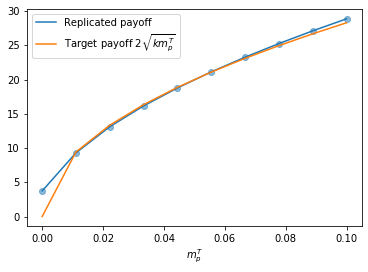
\includegraphics[width=12cm]{figs/replicatedCPM.png}
\centering
\caption{Constant product market value vs replicated value}
\label{fig:CPMReplication}
\end{figure}


   \begin{table}[!ht]
     \caption{Option notional by strike  }\label{tab:OptStrikeWt}
     \centering
     \begin{tabular}{ccc}\toprule
       Strike $K$ & Call notional & Put notional \\ \midrule
       
       0.0125 & 0 & -200     \\
       0.025 & 0 &-70.7    \\
       0.0375 & 0 & -38.5   \\ 
       0.05 & 0 & -25    \\
       0.0625 & -17.8 & 0   \\
       0.075 & -13.6 & 0  \\
       0.0875 & -10.8 & 0 \\
       0.1 & -8.3 & 0 \\
       \toprule
       \addlinespace
     \end{tabular}

   \end{table}
   
\section*{Appendix B. Example: Replicating an option with a CPM} \label{sec:appendixb}
\addcontentsline{toc}{section}{Appendix B: Example: Replicating an option with a CPM}

We simulate 10000 paths of $m_t$ and record the value of the two replicating portfolios for a 30 day at-the-money call on $m^T$ with a starting price $m^0=100$, and constant $20\%$ annual volatility.

Figure \ref{fig:ReplicationComparison} compares replication of the option using a futures and a rebalanced CPM (panel (a) is equation \ref{VCPrime}) to a delta hedge (panel (b)). Figure \ref{fig:CPMBasisPercentile} has the basis between the $V_{C'}^T$ (equation \ref{VCPrime}) and $V_C^T$ (equation \ref{VC}) as a fraction of the option price. 99\% of replications are within 0.7\% of the target portfolio.




\begin{figure}
    \centering
    \subfigure[]{\includegraphics[width=0.6\textwidth]{figs/replicatedWithCPM.png}} 
    \subfigure[]{\includegraphics[width=0.6\textwidth]{figs/replicatedWithDelta.png}} 
    \caption{(a) Replication with CPM (b) Replication with delta }
    \label{fig:ReplicationComparison}
\end{figure}


\begin{figure}[t] 
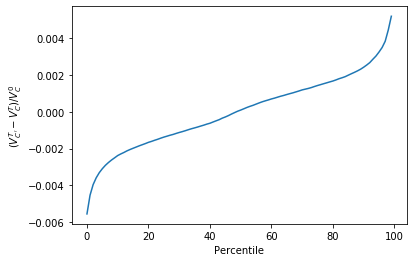
\includegraphics[width=12cm]{figs/CPMBasisPercentile.png}
\centering
\caption{Basis between replication with option greeks and CPM greeks}
\label{fig:CPMBasisPercentile}
\end{figure}

% Note: This is a standard barrier result using reflection and strong markov property but not it doesn't seem to work exactly in sims. What to do?
% Jupyter notebook: MarginsWithPooledInsurance.ipynb



% Extensions:
% Other processes?
% Attack where to manipulate price downwards so that the MP liquidates the collateral too cheaply.


\begin{thebibliography}{}
\bibitem{ang20} Angeris, Guillermo, Hsien-Tang Kao, Rei Chiang, Charlie Noyes, and Tarun Chitra  \textit{An analysis of Uniswap markets}, arXiv preprint arXiv:1911.03380, 2020.


\bibitem{CarrWu09} Carr, P., Wu, L., \textit{Variance risk premiums.} Review of Financial Studies 22, 1311–1341, 2009.

\bibitem{Derman99} Emanuel Derman, Kresimir Demeterfi, Michael Kamal, and Joseph Zou. A guide to volatility
and variance swaps. Journal of Derivatives, 6(4):9–32, 1999.

\bibitem{Zha18} Zhang, Yi, Xiaohong Chen, and Daejun Park \textit{Formal specification of constant product (xy=k) market maker model and implementation}, 2018.

%\bibitem{BS73} Black, Fischer, Scholes, Myron (1973). \textit{The Pricing of Options and Corporate Liabilities}. Journal of Political Economy. 81 (3): 637–654. 

\bibitem{JarrowGreen87} Green R, C., and R.A. Jarrow. \textit{Spanning and completeness in markets with contingent claims.}
Journal of Economic Theory, Vol. 41, No 1, pp. 202-210, 1987.

%\bibitem{Jac2010} Jacobs, Kurt (2010). Stochastic Processes for Physicists. Cambridge University Press. pp. 57–59

%\bibitem{Merton73} Merton, Robert (1973). \textit{Theory of Rational Option Pricing}. Bell Journal of Economics and Management Science. 4 (1): 141–183.


%@article{angeris2019analysis,
%  title={An analysis of Uniswap markets},
%  author={Angeris, Guillermo and Kao, Hsien-Tang and Chiang, Rei and Noyes, %Charlie and Chitra, Tarun},
%  journal={arXiv preprint arXiv:1911.03380},
%  year={2019}


\end{thebibliography}

\end{document}
